\chapter{$\epsilon^{i,\gamma\gamma}_k$ matrices: 2016 and 2017}\label{app:eff_acc}

\begin{figure}[hptb]
  \centering
  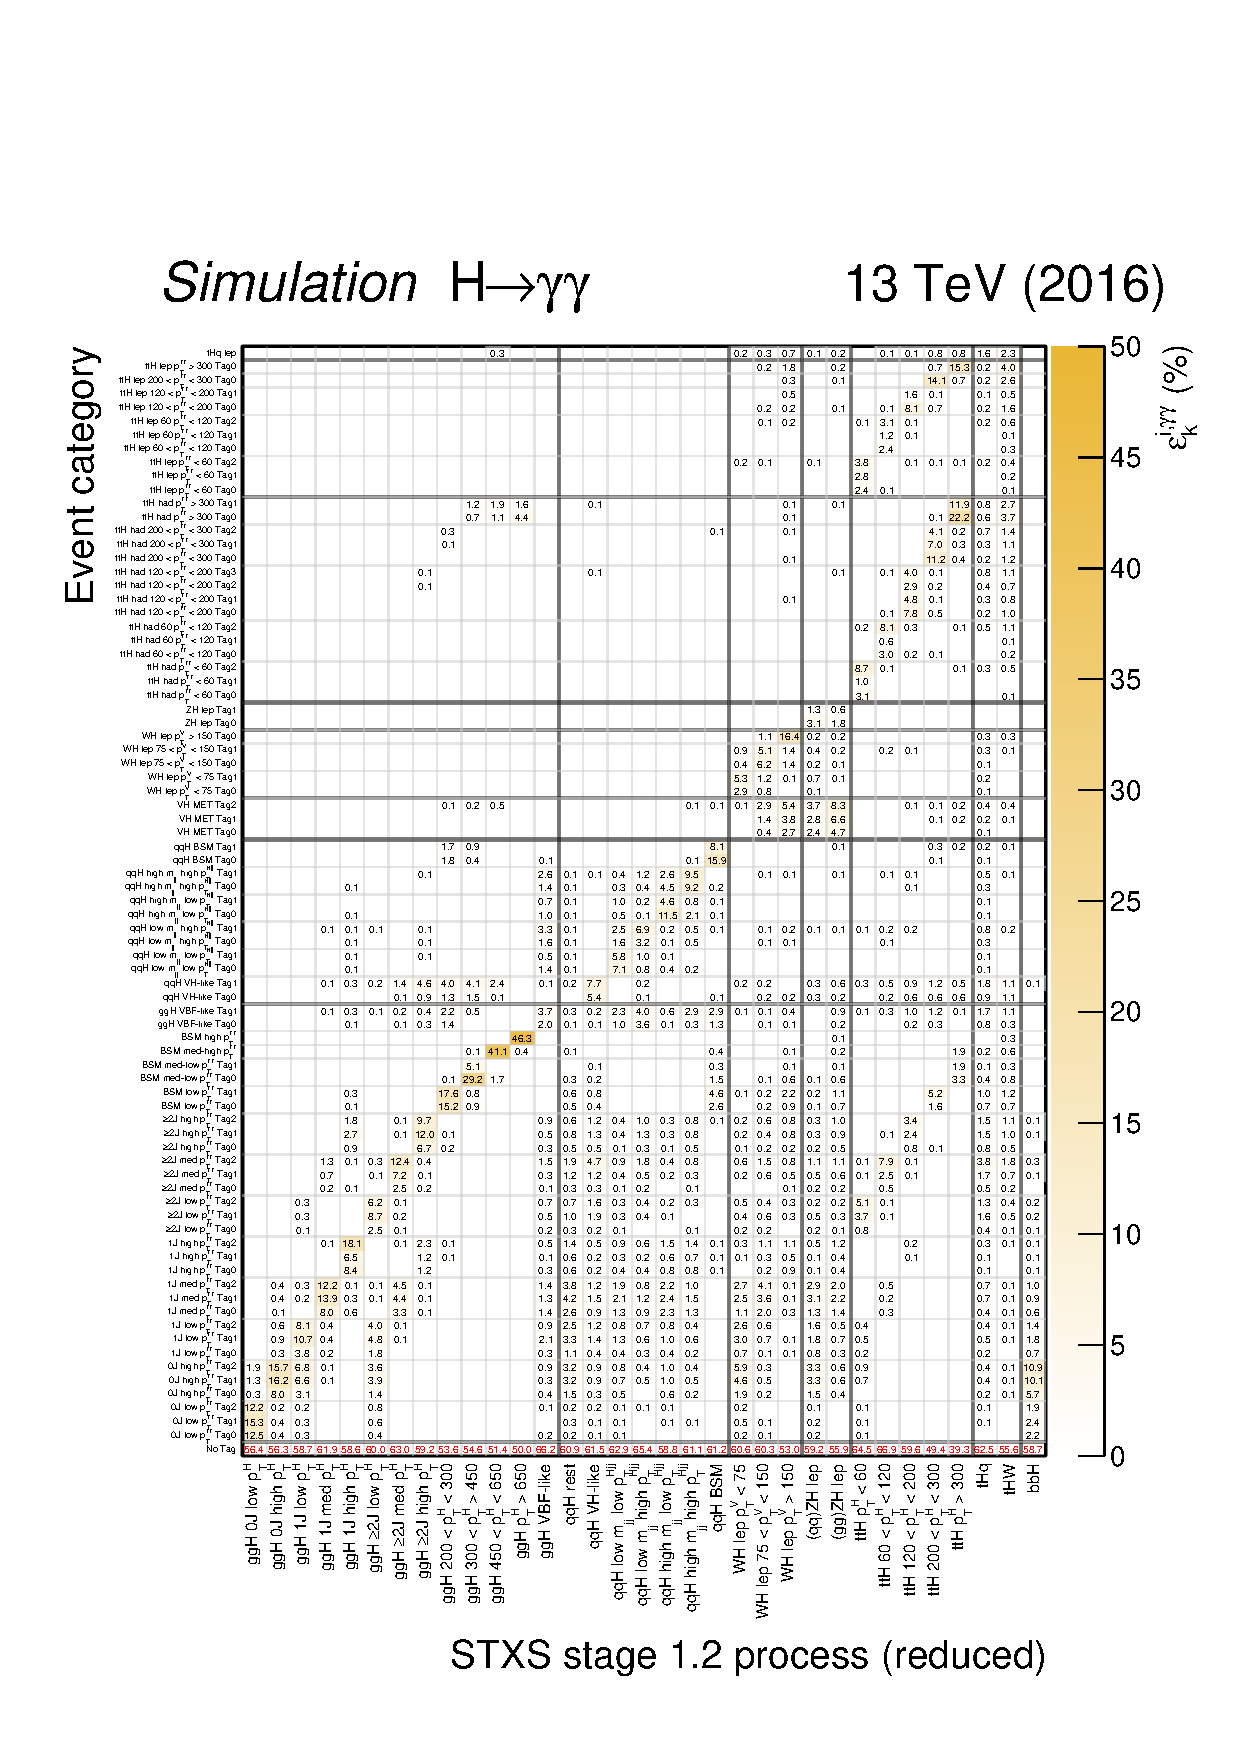
\includegraphics[width=1\textwidth]{Figures/hgg_stats/migrationMatrix_2016_thesis.pdf}
  \caption[Efficiency times acceptance matrix from 2016 simulation]
  {
    A matrix showing the $\epsilon^{i,\gamma\gamma}_{k}$ terms for a reduced set of STXS bins, derived from 2016 simulation. The numbers corresponds to the fraction of the total yield of STXS bin, $i$, landing in analysis category, $k$, expressed as a percentage. Each column therefore sums to 100\%. Entries with values less than 0.05\% are not shown. The bottom row indicates the fraction of events which do not enter a single analysis category. The column labelled as qqH rest includes the contributions from the qqH 0J, qqH 1J, qqH $m_{jj}<60$~GeV and the qqH $120<m_{jj}<350$~GeV STXS bins.
  }
  \label{fig:ea_2016}
\end{figure}

\begin{figure}[hptb]
  \centering
  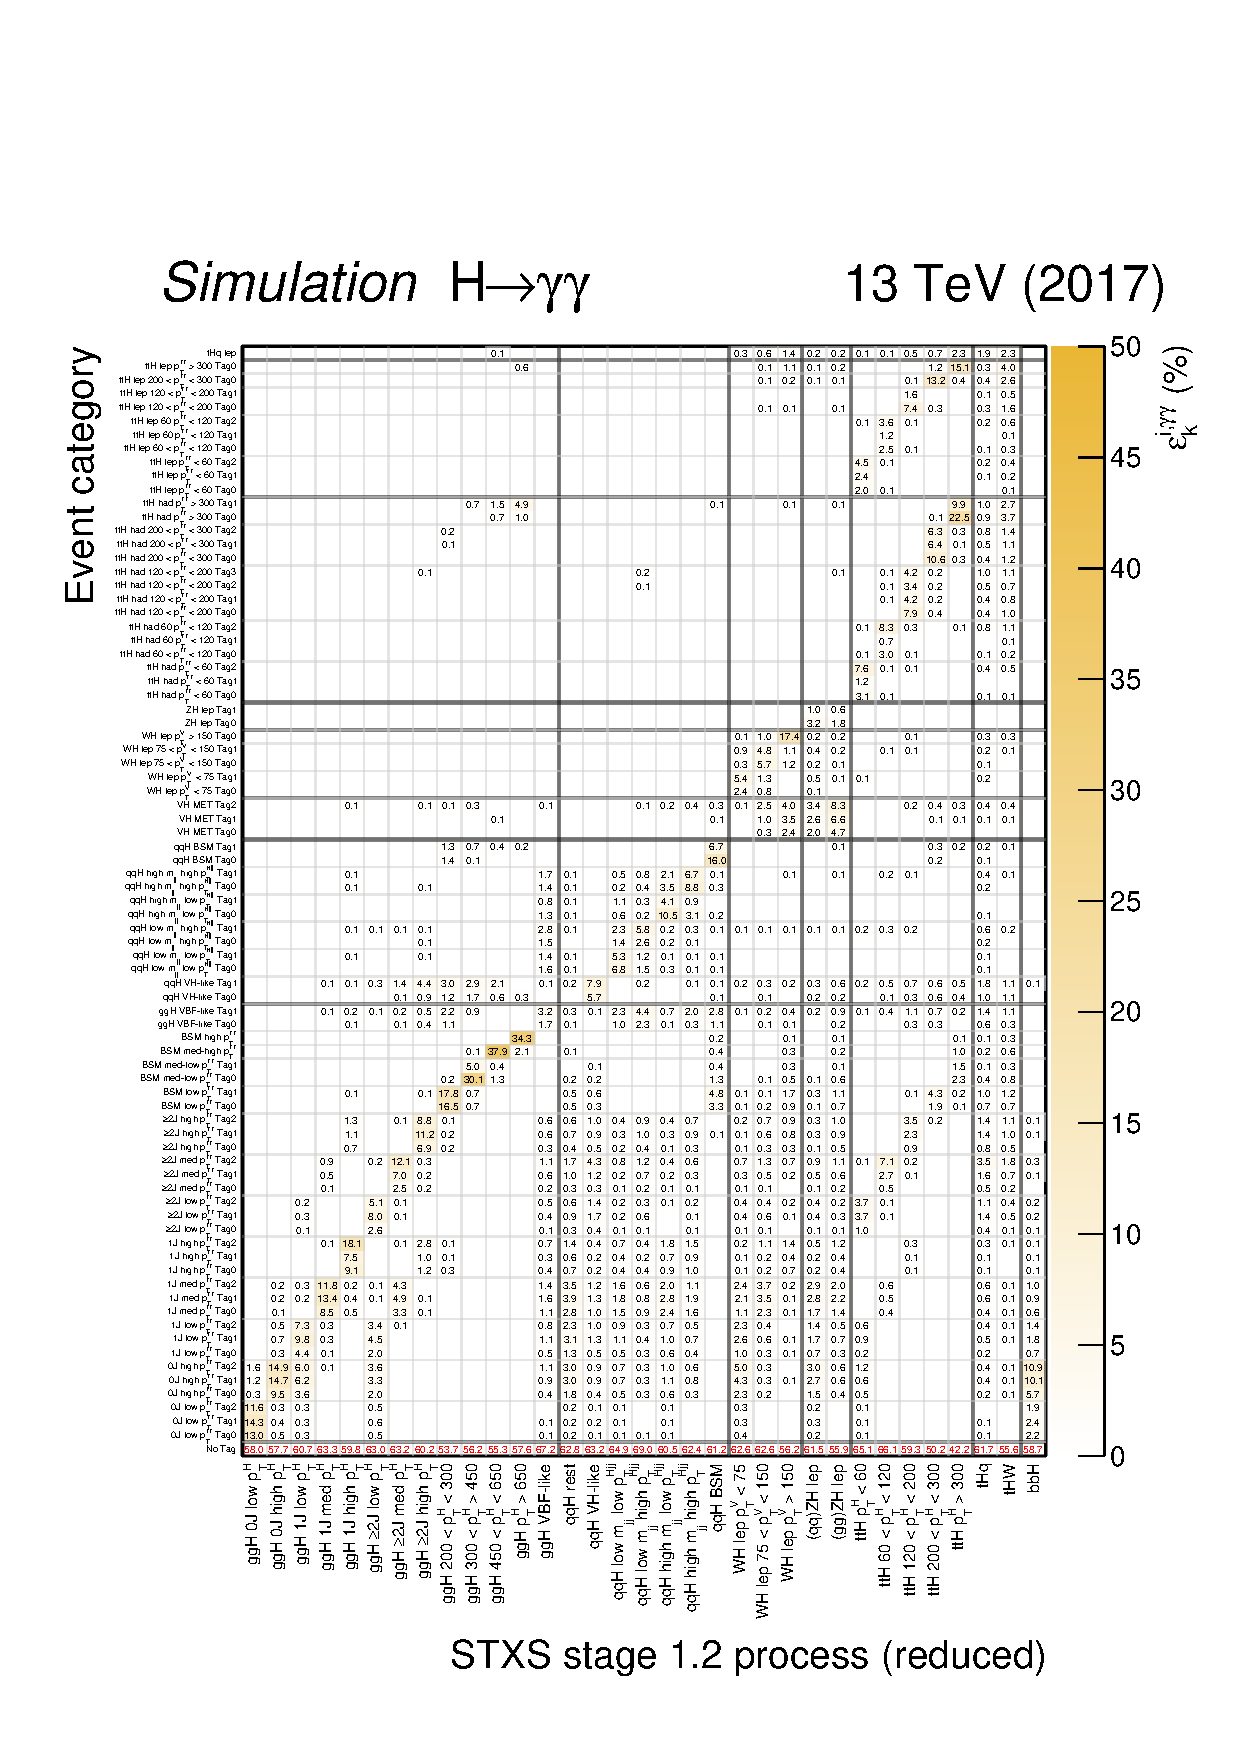
\includegraphics[width=1\textwidth]{Figures/hgg_stats/migrationMatrix_2017_thesis.pdf}
  \caption[Efficiency times acceptance matrix from 2017 simulation]
  {
    A matrix showing the $\epsilon^{i,\gamma\gamma}_{k}$ terms for a reduced set of STXS bins, derived from 2017 simulation. The numbers corresponds to the fraction of the total yield of STXS bin, $i$, landing in analysis category, $k$, expressed as a percentage. Each column therefore sums to 100\%. Entries with values less than 0.05\% are not shown. The bottom row indicates the fraction of events which do not enter a single analysis category. The column labelled as qqH rest includes the contributions from the qqH 0J, qqH 1J, qqH $m_{jj}<60$~GeV and the qqH $120<m_{jj}<350$~GeV STXS bins.
  }
  \label{fig:ea_2017}
\end{figure}